\begin{center}
\Huge
	Pythagoras' sætning
\end{center}

\section*{Pythagoras' sætning}
\stepcounter{section}

Pythagoras' sætning giver en relation mellem sidelængderne i retvinklede trekanter. Vi betragter trekanten
$\triangle ABC$ på Figur \ref{fig:pytte}.
\begin{figure}[H]
	\centering
	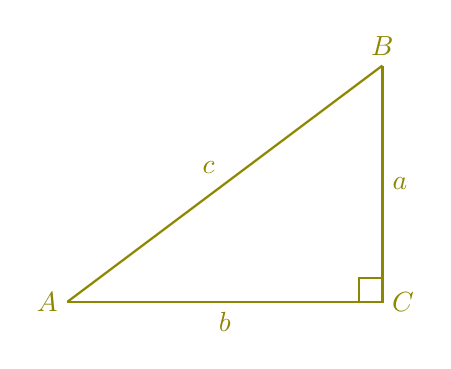
\begin{tikzpicture}
		\draw[color = olive, thick] (0,0) -- (4,0) node[midway, anchor = north] {$b$};
		\draw[color = olive, thick] (0,0) -- (4,3) node[midway, anchor = south east] {$c$};
		\draw[color = olive, thick] (4,0) -- (4,3) node[midway, anchor = west] {$a$};
		\draw[color = olive, thick] (3.7,0) rectangle (4,0.3);
		\node[color = olive, anchor = east] at (0,0) {$A$};
		\node[color = olive, anchor = west] at (4,0) {$C$};
		\node[color = olive, anchor = south] at (4,3) {$B$};
	\end{tikzpicture}
	\caption{Retvinklet trekant.}
	\label{fig:pytte}
\end{figure}
\begin{setn}[Pythagoras]
	For retvinklede trekanter som den, der ses på Figur \ref{fig:pytte} gælder det, at 
	\begin{align*}
		a^2 + b^2 = c^2.
	\end{align*}
\end{setn}
\begin{proof}
	Opgave 1, 2, 3 og 4.
\end{proof}

Vi skal i dag bevise denne sætning på tre forskellige måder. Både geometrisk og algebraisk. 

\newpage
\subsection*{Opgave 1}
Vi ønsker at bevise Pythagoras' sætning geometrisk. 

\begin{enumerate}[label=\roman*)]
	\item Læg brikkerne, så du får to kvadrater med hver sidelængde $a + b$. Den farvede side skal vende op.
	\item Hvad er arealet af det blå område for hver af de to kvadrater? Hvorfor er dette et bevis for
	 Pythagoras' sætning?
\end{enumerate}

\newpage

\subsection*{Opgave 2}
Vi ønsker nu at bevise Pythagoras' sætning algebraisk (med bogstaver). Vi betragter derfor Figur \ref{fig:algebraisk}.

\begin{figure}[H]
	\centering
	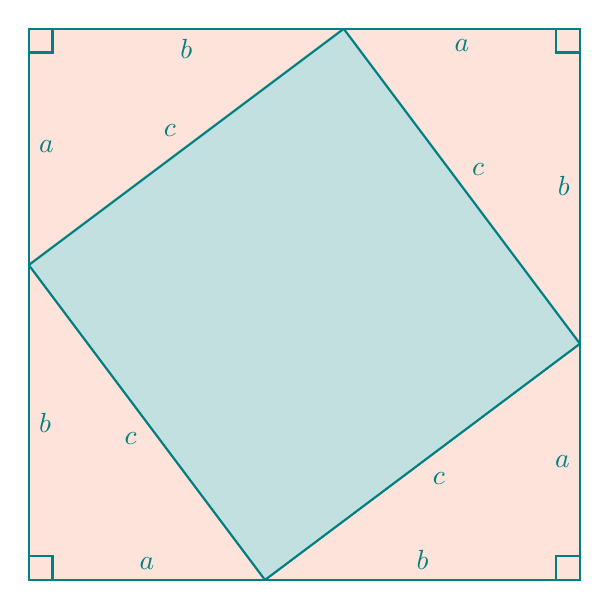
\begin{tikzpicture}
		%color_triangle
		\fill[color = Melon!60, opacity = 0.4] (0,0) -- (3,0) -- (0,4) -- cycle;
		\fill[color = Melon!60, opacity = 0.4] (0,4) -- (4,7) -- (0,7) -- cycle;
		\fill[color = Melon!60, opacity = 0.4] (4,7) -- (7,3) -- (7,7) -- cycle;
		\fill[color = Melon!60, opacity = 0.4] (3,0) -- (7,0) -- (7,3) -- cycle;
		%color_square
		\fill[color = teal!60, opacity = 0.4] (3,0) -- (7,3) -- (4,7) -- (0,4) -- cycle;
		%perimeter
		\draw[color = teal, thick] (0,0) -- (3,0) node[midway, anchor = south] {$a$};
		\draw[color = teal, thick] (3,0) -- (7,0) node[midway, anchor = south] {$b$};
		\draw[color = teal, thick] (0,0) -- (0,4) node[midway, anchor = west] {$b$};
		\draw[color = teal, thick] (0,4) -- (0,7) node[midway, anchor = west] {$a$};
		\draw[color = teal, thick] (0,7) -- (4,7) node[midway, anchor = north] {$b$};
		\draw[color = teal, thick] (4,7) -- (7,7) node[midway, anchor = north] {$a$};
		\draw[color = teal, thick] (7,7) -- (7,3) node[midway, anchor = east] {$b$};
		\draw[color = teal, thick] (7,3) -- (7,0) node[midway, anchor = east] {$a$};
		%hypotenuse
		\draw[color = teal, thick] (3,0) -- (0,4) node[midway, anchor = north east] {$c$};
		\draw[color = teal, thick] (0,4) -- (4,7) node[midway, anchor = south east] {$c$};
		\draw[color = teal, thick] (4,7) -- (7,3) node[midway, anchor = south west] {$c$};
		\draw[color = teal, thick] (7,3) -- (3,0) node[midway, anchor = north west] {$c$};
		%angles
		\draw[color = teal, thick] (0,0) rectangle (0.3,0.3);
		\draw[color = teal, thick] (0,7) rectangle (0.3,6.7);
		\draw[color = teal, thick] (7,7) rectangle (6.7,6.7);
		\draw[color = teal, thick] (7,0) rectangle (6.7,0.3);
	\end{tikzpicture}
	\caption{Algebraisk bevis for Pythagoras' sætning.}
	\label{fig:algebraisk}
\end{figure}
\begin{enumerate}[label=\roman*)]
	\item Opskriv arealet af kvadratet på Figur \ref{fig:algebraisk} som summen af arealet af de fire trekanter
	samt det lille kvadrat. 
	\item Opskriv arealet af kvadratet på Figur \ref{fig:algebraisk} ved brug af kvadratets sidelængder.
	\item Sæt disse to udtryk lig hinanden. 
	\item Hæv parentesen (husk at bruge en kvadratsætning).
	\item Reducer udtrykket og sammenlign med Pythagoras sætning. 
\end{enumerate}

\newpage

\subsection*{Opgave 3}
Vi vil bevise Pythagoras sætning algebraisk, men på en anden måde. Betragt derfor kvadratet på Figur \ref{fig:algebraisk2}.

\begin{figure}[H]
	\centering
	
	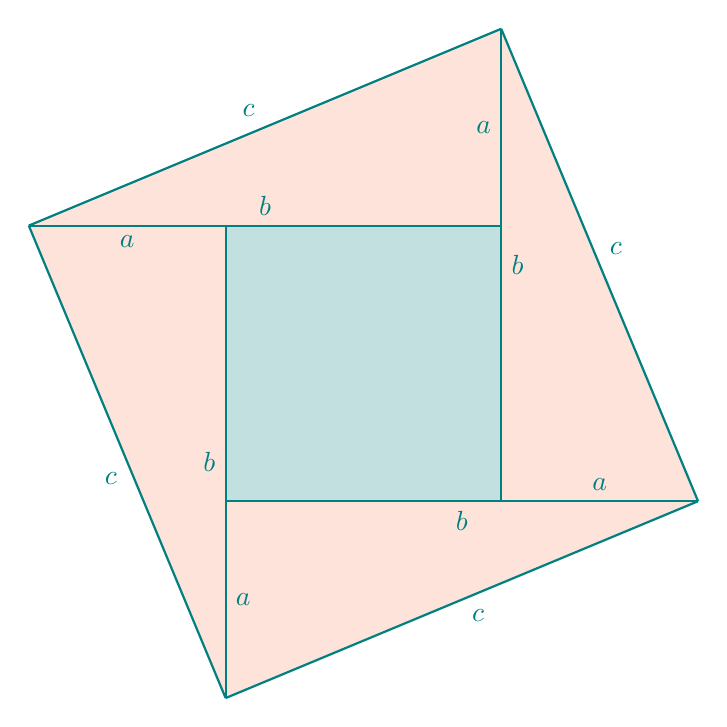
\begin{tikzpicture}
	%color
	\fill[color = Melon!60, opacity = 0.4] (0,0) -- (0,2.5) -- (6,2.5) -- cycle;
	\fill[color = Melon!60, opacity = 0.4] (0,0) -- (0,6) -- (-2.5,6) -- cycle;
	\fill[color = Melon!60, opacity = 0.4] (-2.5,6) -- (3.5,8.5) -- (3.5,6) -- cycle;
	\fill[color = Melon!60, opacity = 0.4] (3.5,8.5) -- (3.5,2.5) -- (6,2.5) -- cycle;
	\fill[color = teal!60, opacity = 0.4] (0,2.5) -- (3.5,2.5) -- (3.5,6) -- (0,6) -- cycle;
	%perimeter
	\draw[color = teal, thick] (0,0) -- (6,2.5) node[midway, anchor = north west] {$c$};
	\draw[color = teal, thick] (6,2.5) -- (3.5,8.5) node[midway, anchor = south west] {$c$};
	\draw[color = teal, thick] (3.5,8.5) -- (-2.5,6) node[midway, anchor = south east] {$c$};
	\draw[color = teal, thick] (-2.5,6) -- (0,0) node[midway, anchor = north east] {$c$};
	%Kateter
	\draw[color = teal, thick] (0,0) -- (0,2.5) node[midway, anchor = west] {$a$};
	\draw[color = teal, thick] (0,0) -- (0,6) node[midway, anchor = east] {$b$};
	\draw[color = teal, thick] (-2.5,6) -- (0,6) node[midway, anchor = north] {$a$};
	\draw[color = teal, thick] (-2.5,6) -- (3.5,6) node[midway, anchor = south] {$b$};
	\draw[color = teal, thick] (3.5,8.5) -- (3.5,6) node[midway, anchor = east] {$a$};
	\draw[color = teal, thick] (3.5,8.5) -- (3.5,2.5) node[midway, anchor = west] {$b$};
	\draw[color = teal, thick] (6,2.5) -- (3.5,2.5) node[midway, anchor = south] {$a$};
	\draw[color = teal, thick] (6,2.5) -- (0,2.5) node[midway, anchor = north] {$b$};
	\end{tikzpicture}
	\caption{Andet algebraisk bevis for Pythagoras' sætning}
	\label{fig:algebraisk2}
\end{figure}
\begin{enumerate}[label=\roman*)]
	\item Afgør, hvor lange sidelængderne er i det lille kvadrat på Figur \ref{fig:algebraisk2}.
	\item Opskriv arealet af kvadratet på Figur \ref{fig:algebraisk2} som summen af arealet af de fire
	 trekanter samt det lille kvadrat.
	\item Opskriv arealet af kvadratet på Figur \ref{fig:algebraisk2} ved brug af kvadratets sidelængder.
	\item Sæt disse to udtryk lig hinanden. 
	\item Hæv parentesen (husk at bruge en kvadratsætning).
	\item Reducer udtrykket og sammenlign med Pythagoras sætning. 
\end{enumerate}

\newpage

\subsection*{Opgave 4}
Vi mangler at redegøre for en detalje i beviserne. I Figur \ref{fig:algebraisk} skal vi redegøre for, at vinklerne i det blå kvadrat rent faktisk er $90^\circ$. I Figur \ref{fig:algebraisk2} skal vi redegøre for, at det store kvadrat har rette vinkler. 
\begin{enumerate}[label=\roman*)]
	\item Udnyt, at vinkelsummen i en trekant er $180^\circ$ samt at en ret linje dækker over 180 grader til at 
	argumentere for, at vinklerne i det blå kvadrat i Figur \ref{fig:algebraisk} er $90^\circ$.
	\item Udnyt, at vinkelsummen i en trekant er $180^\circ$ til at redegøre for, at Figur \ref{fig:algebraisk2}
	er et kvadrat. 
\end{enumerate}

\newpage 

\begin{center}
	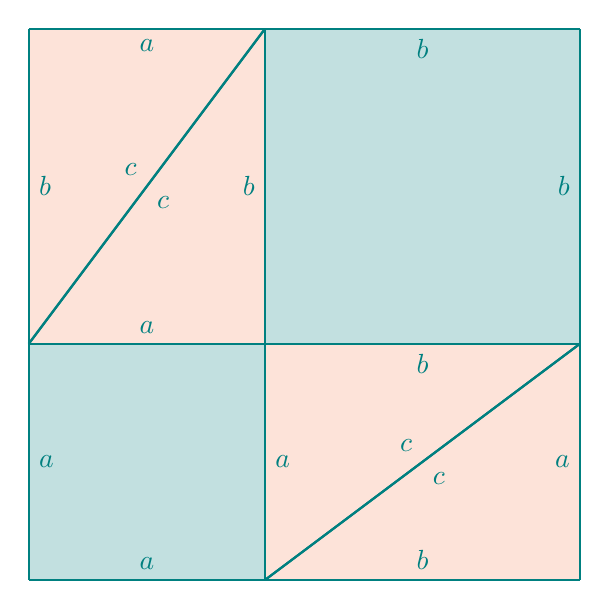
\begin{tikzpicture}
		%color		
		\fill[color = Melon!60,opacity = 0.4] (3,0) -- (7,0) -- (7,3) -- (3,3) -- cycle;
		\fill[color = Melon!60,opacity = 0.4] (3,3) -- (3,7) -- (0,7) -- (0,3) -- cycle;
		\fill[color = teal!60,opacity = 0.4] (0,0) -- (3,0) -- (3,3) -- (0,3) -- cycle;
		\fill[color = teal!60,opacity = 0.4] (3,3) -- (7,3) -- (7,7) -- (3,7) -- cycle;
		%Perimeter
		\draw[color = teal, thick] (0,0) -- (3,0) node[midway, anchor = south] {$a$};
		\draw[color = teal, thick] (3,0) -- (7,0) node[midway, anchor = south] {$b$};
		\draw[color = teal, thick] (0,0) -- (0,3) node[midway, anchor = west] {$a$};
		\draw[color = teal, thick] (0,3) -- (0,7) node[midway, anchor = west] {$b$}; 
		\draw[color = teal, thick] (0,7) -- (3,7) node[midway, anchor = north] {$a$};
		\draw[color = teal, thick] (3,7) -- (7,7) node[midway, anchor = north] {$b$};
		\draw[color = teal, thick] (7,0) -- (7,3) node[midway, anchor = east] {$a$};
		\draw[color = teal, thick] (7,3) -- (7,7) node[midway, anchor = east] {$b$};		
		 %cross
		\draw[color = teal, thick] (3,0) -- (3,3) node[midway, anchor = west] {$a$};
		\draw[color = teal, thick] (3,3) -- (3,7) node[midway, anchor = east] {$b$};
		\draw[color = teal, thick] (0,3) -- (3,3) node[midway, anchor = south] {$a$};
		\draw[color = teal, thick] (3,3) -- (7,3) node[midway, anchor = north] {$b$};
		%hypotenuse
		\draw[color = teal, thick] (0,3) -- (3,7) node[midway, anchor = south east] {$c$};
		\draw[color = teal, thick] (0,3) -- (3,7) node[midway, anchor = north west] {$c$};
		\draw[color = teal, thick] (3,0) -- (7,3) node[midway, anchor = south east] {$c$};
		\draw[color = teal, thick] (3,0) -- (7,3) node[midway, anchor = north west] {$c$};
		%color
	\end{tikzpicture}
\end{center} 

\begin{center}
	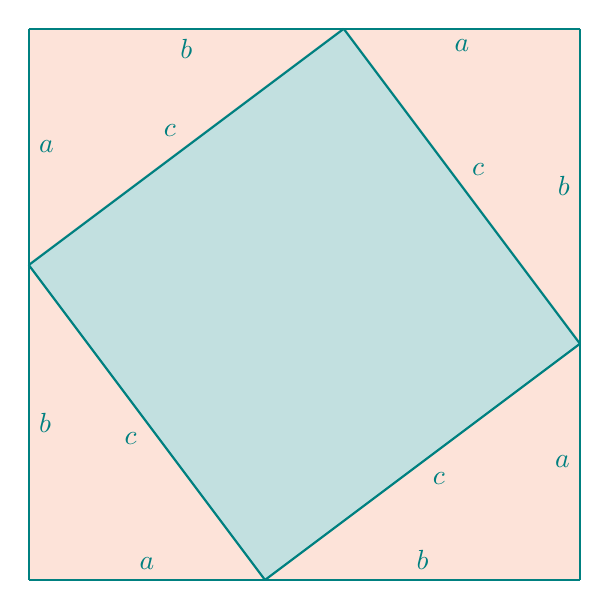
\begin{tikzpicture}
		%color_triangle
		\fill[color = Melon!60, opacity = 0.4] (0,0) -- (3,0) -- (0,4) -- cycle;
		\fill[color = Melon!60, opacity = 0.4] (0,4) -- (4,7) -- (0,7) -- cycle;
		\fill[color = Melon!60, opacity = 0.4] (4,7) -- (7,3) -- (7,7) -- cycle;
		\fill[color = Melon!60, opacity = 0.4] (3,0) -- (7,0) -- (7,3) -- cycle;
		%color_square
		\fill[color = teal!60, opacity = 0.4] (3,0) -- (7,3) -- (4,7) -- (0,4) -- cycle;
		%perimeter
		\draw[color = teal, thick] (0,0) -- (3,0) node[midway, anchor = south] {$a$};
		\draw[color = teal, thick] (3,0) -- (7,0) node[midway, anchor = south] {$b$};
		\draw[color = teal, thick] (0,0) -- (0,4) node[midway, anchor = west] {$b$};
		\draw[color = teal, thick] (0,4) -- (0,7) node[midway, anchor = west] {$a$};
		\draw[color = teal, thick] (0,7) -- (4,7) node[midway, anchor = north] {$b$};
		\draw[color = teal, thick] (4,7) -- (7,7) node[midway, anchor = north] {$a$};
		\draw[color = teal, thick] (7,7) -- (7,3) node[midway, anchor = east] {$b$};
		\draw[color = teal, thick] (7,3) -- (7,0) node[midway, anchor = east] {$a$};
		%hypotenuse
		\draw[color = teal, thick] (3,0) -- (0,4) node[midway, anchor = north east] {$c$};
		\draw[color = teal, thick] (0,4) -- (4,7) node[midway, anchor = south east] {$c$};
		\draw[color = teal, thick] (4,7) -- (7,3) node[midway, anchor = south west] {$c$};
		\draw[color = teal, thick] (7,3) -- (3,0) node[midway, anchor = north west] {$c$};
	\end{tikzpicture}
\end{center}
